\appendix

\chapter{Anexe}

\section{Figuri}

\begin{figure}[h]
	\centering
	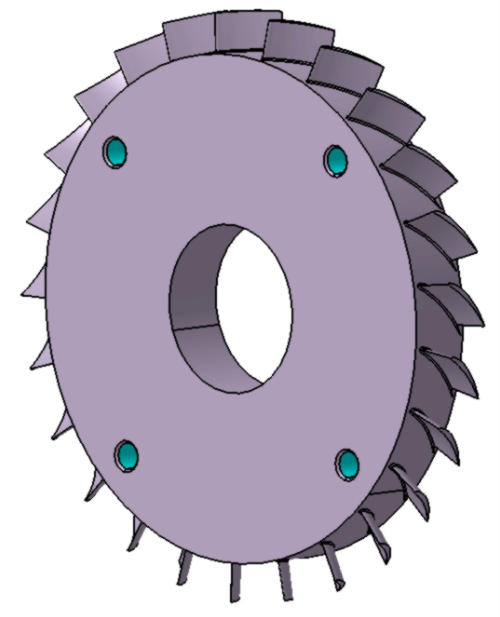
\includegraphics[scale=0.4]{figures/stator-CAD.PNG}
	\caption{Stator}
	\label{Stator}
\end{figure}

\begin{figure}[h]
	\centering
	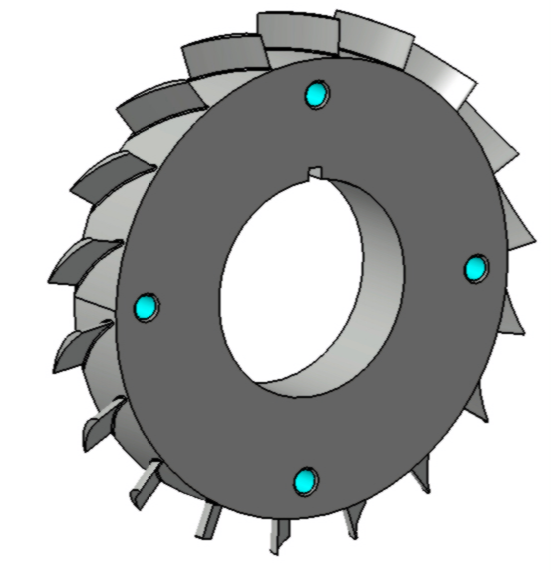
\includegraphics[scale=0.4]{figures/rotor-CAD.PNG}
	\caption{Rotor}
	\label{Rotor}
\end{figure}

\clearpage


\begin{figure}[h]
	\centering
	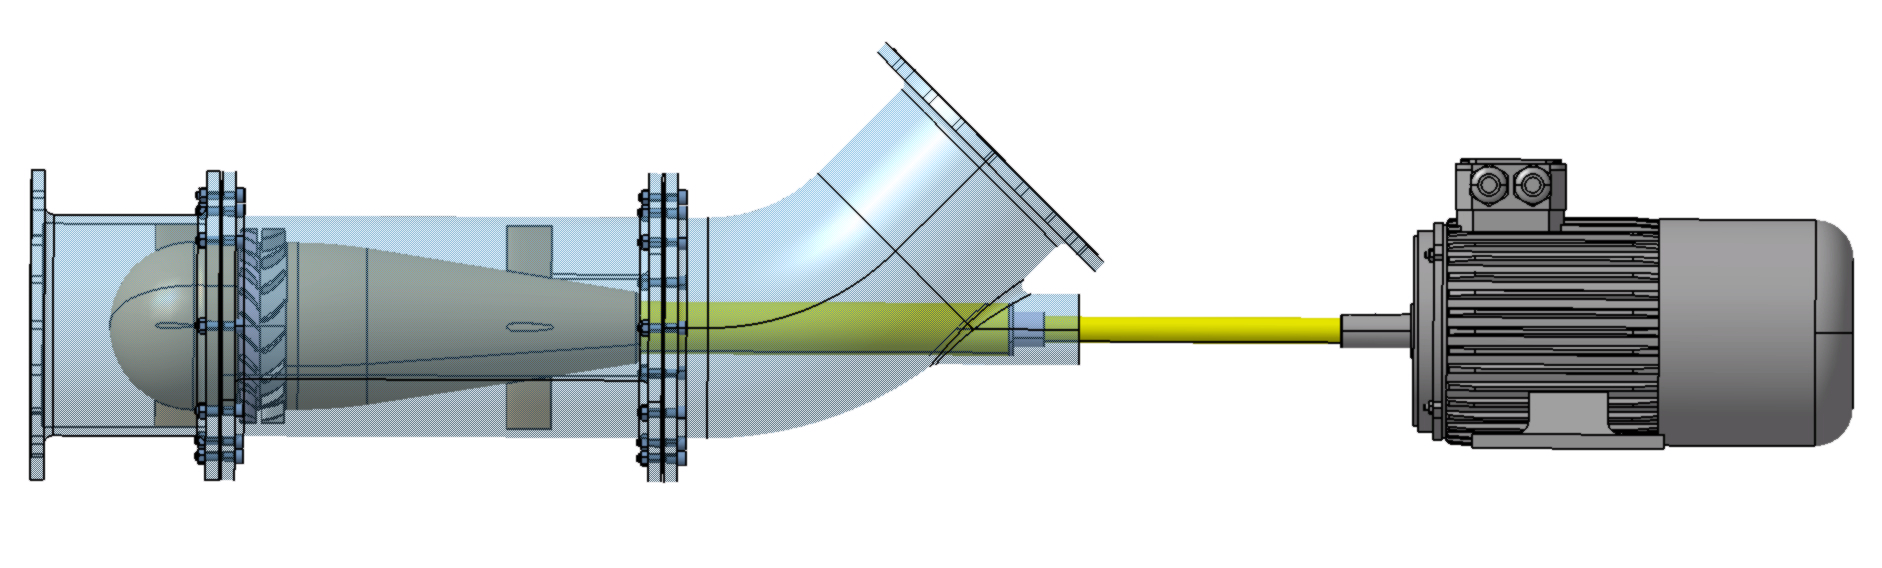
\includegraphics[scale=0.4, angle = -90]{figures/assy.jpg}
	\caption{Ansamblu turbină AXENT}
	\label{Ansamblu turbină AXENT}
\end{figure}

\clearpage


\section{Programe Fortran de calcul}

\subsection{Rezolvarea ecuației polinomiale cubice}

\lstinputlisting[language=Fortran]{code/free-swirl-stag.for}

\clearpage


\subsection{Setarea rețelei și a formei inițiale a paletei}

\lstinputlisting[language=Fortran]{code/bladesetup.for}

\clearpage


\subsection{Corecția iterativă a formei și pantei paletei subțiri}

\lstinputlisting[language=Fortran]{code/bladeupdate.for}

\clearpage


\subsection{Calculul modulului vitezei pe fețele paletei}

\lstinputlisting[language=Fortran]{code/bladevelocity.for}

\clearpage


\begin{comment}
\subsection{Subrutina de calcula a valorii minime a unei funcții cu variabile multiple}

\lstinputlisting[language=Fortran]{code/bobyqa.for}

\clearpage
\end{comment}


\subsection{Design pentru paleta subțire cu o viteză maximă minimă}

\lstinputlisting[language=Fortran]{code/thinbladecascade.for}

\clearpage


\subsection{Adăugare funcție de grosime}

\lstinputlisting[language=Fortran]{code/thickblade.for}

\clearpage


\section{Prezentare lucrare științifică}

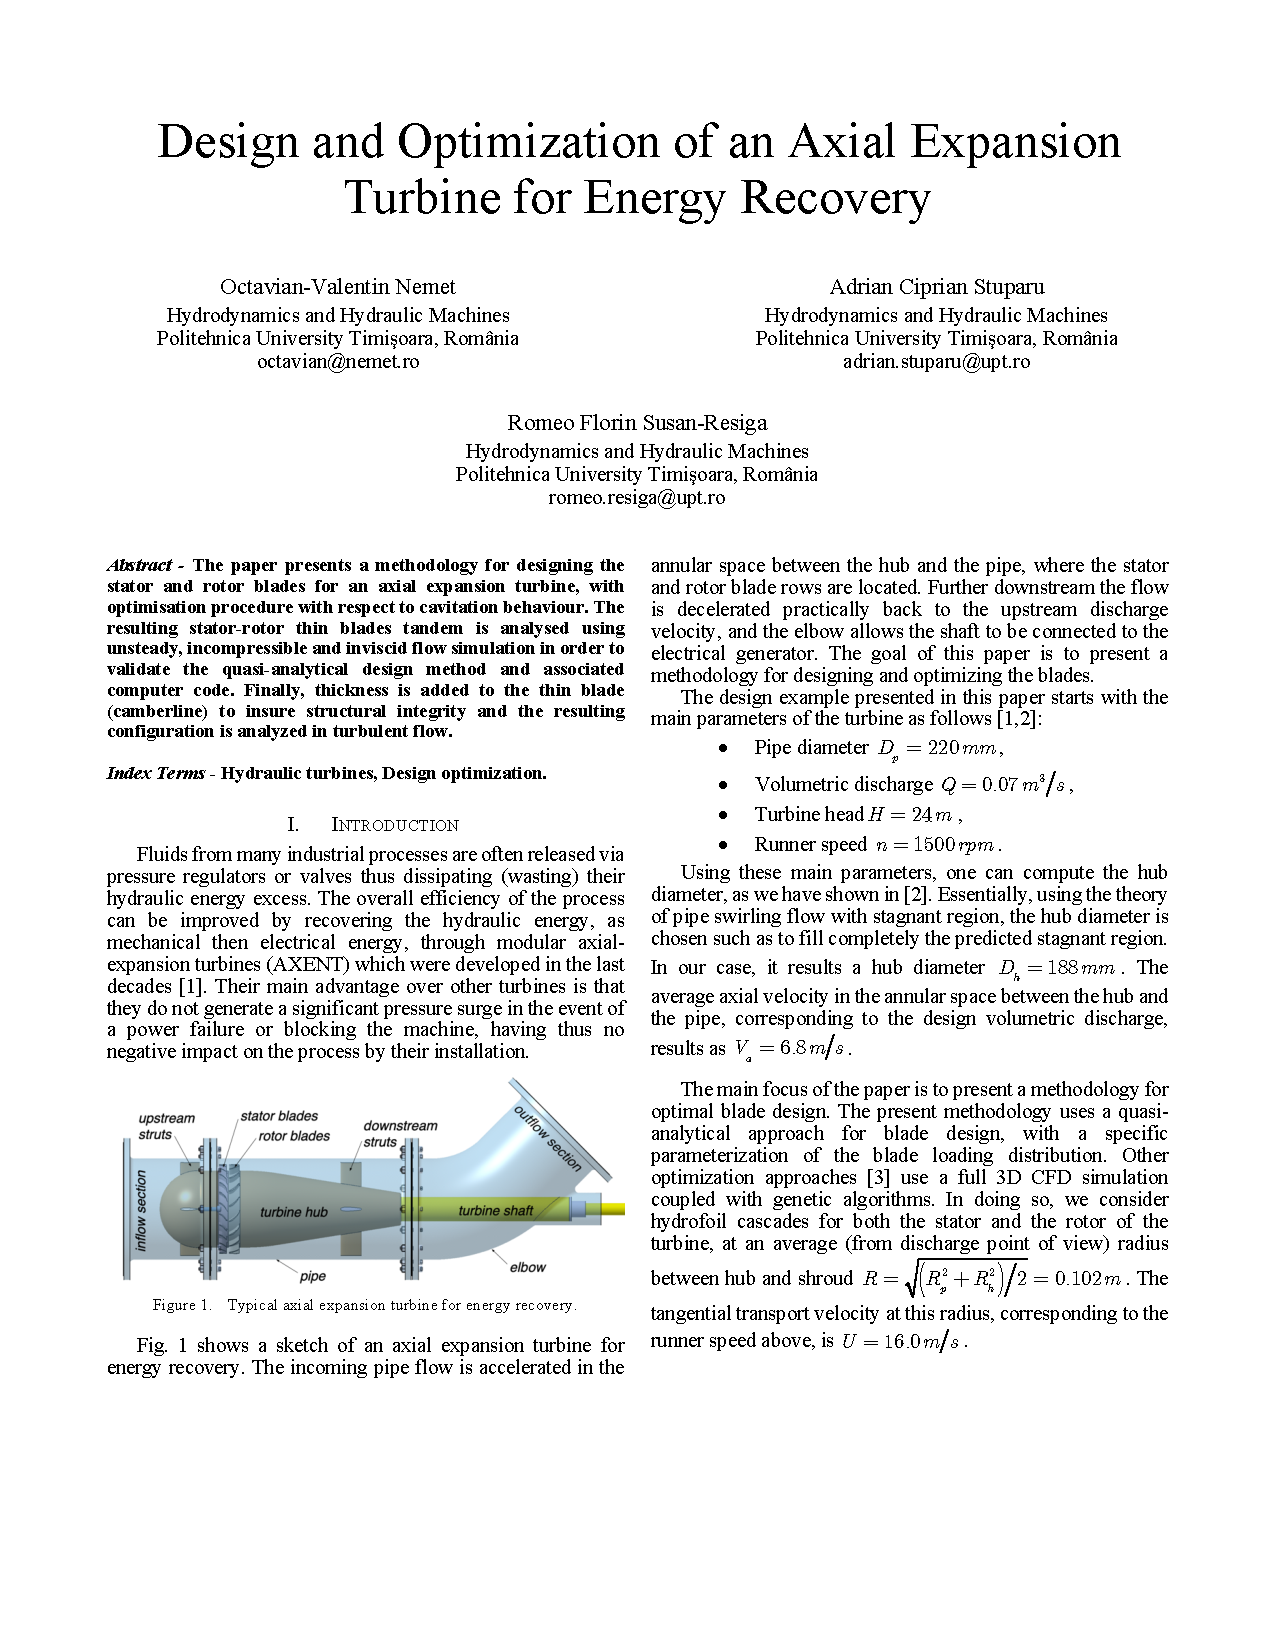
\includepdf[pages={1-}]{pages/AXENT_CIEM2019_Full_Paper_rev08.pdf}

\clearpage